\documentclass[12pt,a4paper]{article}
\usepackage{graphicx}
\usepackage{wrapfig}

\title{Praktikum Physik - Tr\"agheitsmoment}
\author{Simon Marti, Patricia Schwab, Mirco Kocher}
\date{02.03.2012}

\begin{document}
\maketitle

%%
% Ziel
%%
\section*{Ziel}
Berechnung der Tr\"agheitsmomente unterschiedlicher K\"orper durch Messung der Schwingungsperiode und Verifizierung des Satzes von Steiner.

%%
% Motivation
%%
\section*{Motivation}
Der Versuch des Tr\"agheitsmoments eignet sich gut als Einstieg ins Physikpraktikum. Ausserdem kann mit den gemessenen Daten eine umfassende Fehlerrechnung durchgef\"uhrt werden.

%%
% Theorie
%%
\section*{Theorie}
Das Tr\"agheitsmoment $J_{Quader}$ eines homogenen Quaders der Masse $m$ mit L\"ange $l$ und Breite $b$ ist durch folgende Formel gegeben:
\begin{equation}
 J_{Quader} = \frac{m}{12}(l^2 + b^2)
\end{equation}
Eine homogenen Scheibe der Masse $m$ mit Radius $R$ hat folgendes Tr\"agheitsmoment $J_{Scheibe}$:
\begin{equation}
J_{Scheibe} = \frac{1}{2}mR^2
\end{equation}
Das Tr\"agheitsmoment $J$ eines beliebigen K\"orpers bei einer Periodenschwingungsdauer von $T$ und Federkonstante $k$  l\"asst sich folgendermassen bestimmen:
\begin{equation} \label{eq:k}
J = \frac{T^2k}{4\pi^2}
\end{equation}

%%
% Experiment
%%
\section*{Experiment I}

% Aufbau und Ablauf
\subsection*{Aufbau und Ablauf}
\subsubsection*{Teilaufgabe I}
\begin{wrapfigure}{r}{8cm}
\vspace{-50pt}
\centering
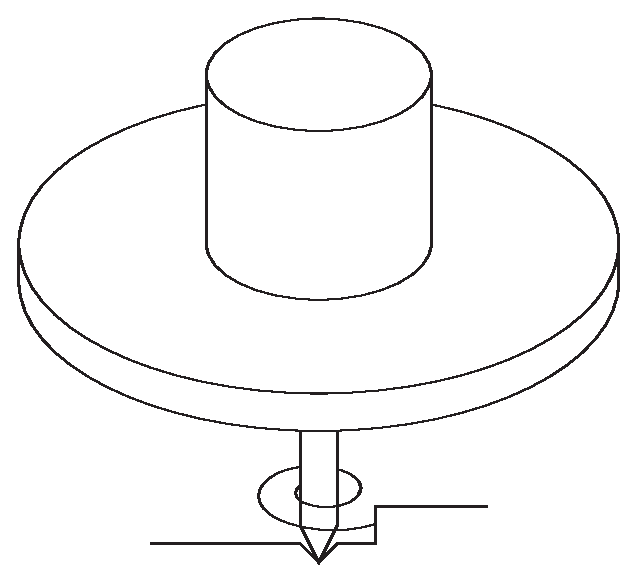
\includegraphics[width=6cm]{illustration11.pdf}
\end{wrapfigure}
Auf einem Drehtisch der durch eine Spiralfeder an der Drehachse als Drehpendel fungiert wird ein Zylinder ($m$ = 600g) zentral befestigt und die Schwingdauer $T$ mithilfe einer Stopp\-uhr bestimmt. Um den Fehler dieser Messmethode zu minimieren werden zehn Messungen durchgef\"uhrt und jeweils $10T$ gemessen.

\subsubsection*{Teilaufgabe II}
\begin{wrapfigure}{r}{8cm}
\vspace{-50pt}
\centering
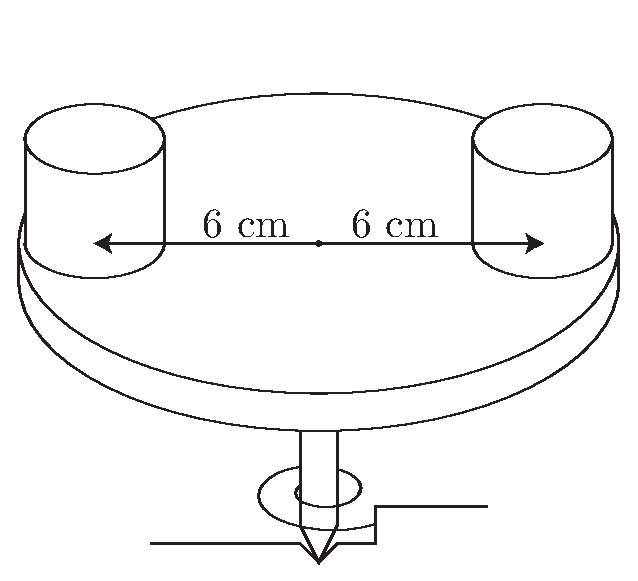
\includegraphics[width=6cm]{illustration12.pdf}
\end{wrapfigure}
Auf dem Drehtisch werden zwei Zylinder ($m$ = 300g) so montiert, dass sie sich direkt gegen\"uber stehen und ihr Zentrum 6cm von der Drehachse entfernt ist. Die Periode $T$ wird dann gem\"ass Teilaufgabe I gemessen.

% Rohdaten
\subsection*{Rohdaten}
\subsubsection*{Teilaufgabe I}
\begin{tabular}{|l|l|l|l|l|l|l|l|l|l|}
\hline
$T_{1}$&$T_{2}$&$T_{3}$&$T_{4}$&$T_{5}$&$T_{6}$&$T_{7}$&$T_{8}$&$T_{9}$&$T_{10}$\\
\hline
13.0s&12.9s&12.9s&12.95s&12.9s&13.0s&12.8s&12.85s&12.95s&12.9s\\
\hline
\end{tabular}

\subsubsection*{Teilaufgabe II}
\begin{tabular}{|l|l|l|l|l|l|l|l|l|l|}
\hline
$T_{1}$&$T_{2}$&$T_{3}$&$T_{4}$&$T_{5}$&$T_{6}$&$T_{7}$&$T_{8}$&$T_{9}$&$T_{10}$\\
\hline
25.5s&25.1s&25.1s&25.05s&25.25s&25.55s&25.3s&25.3s&25.55s&25.45s\\
\hline
\end{tabular}

\subsection*{Fehlerrechnung}
\[ s_{T_0} = s_{T_6} = 0.05\mbox{s} \]
\[ {s_k}^2 = \left( \frac{\partial k}{\partial T_6} \right)^2 {s_{T_0}}^2 + \left( \frac{\partial k}{\partial T_0} \right)^2 {s_{T_6}}^2 = \frac{0.64\pi^4m^2d^4}{({T_6}^2-{T_0}^2)^3} \]
\[ \Rightarrow s_k = 0.00083\mbox{Nm}^{-1} \]

% Auswertung
\subsection*{Auswertung}
\[ 10\overline{T}_0 = 12.92\mbox{s} \Rightarrow \overline{T}_0 = (1.29 \pm 0.05) \mbox{s} \]
\[ 10\overline{T}_6 = 25.32\mbox{s} \Rightarrow \overline{T}_6 = (2.53 \pm 0.05) \mbox{s} \]
Mit diesen beiden Werten l\"asst sich nach Formel \ref{eq:k} die Federkonstante $k$ berechnen:
\[ k = \frac{8md^2\pi^2}{{T_6}^2 - {T_0}^2} = (0.01799 \pm 0.00083) \mbox{Nm}^{-1} \]

\newpage
\section*{Experiment II}
% Aufbau und Ablauf
\subsection*{Aufbau und Ablauf}
\begin{center}
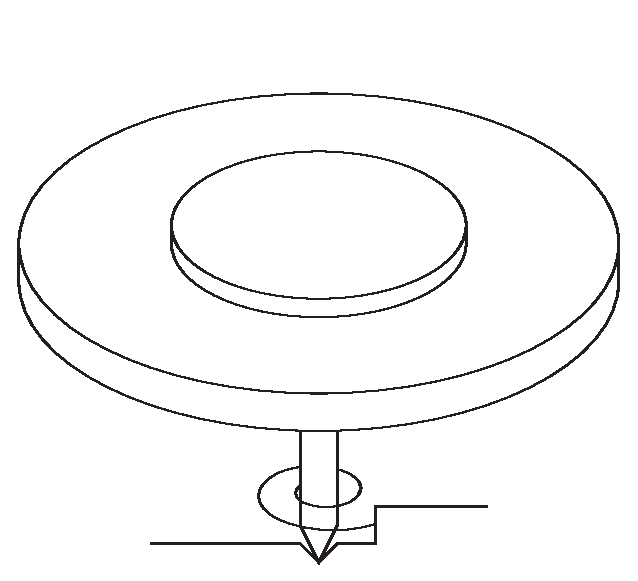
\includegraphics[width=6cm]{illustration21.pdf}
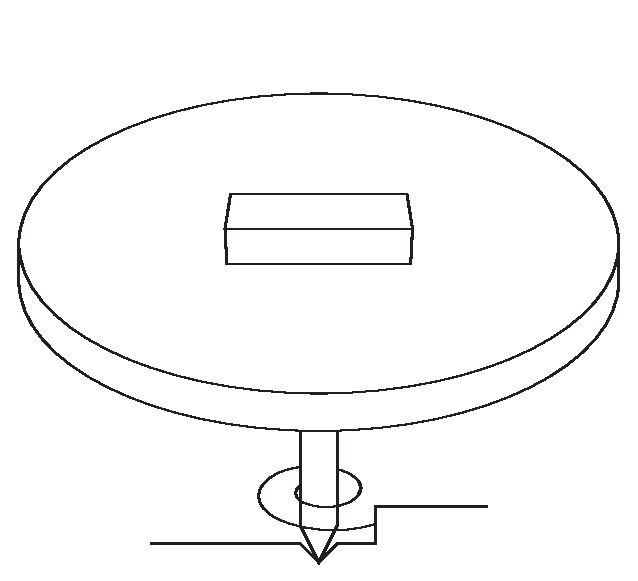
\includegraphics[width=6cm]{illustration22.pdf}
\end{center}
Auf dem Drehtisch werden nacheinander eine Scheibe ($m$ = 300g, $r$=5cm) und ein Quader ($a$ = 2cm, $b$ = 7cm, $m$ = 235g) zentral montiert und die Periode $T$ wie zuvor gemessen. Zus\"atzlich wird die Periode des leeren Tisches gemessen um dessen Tr\"agheitsmoment bestimmen zu k\"onnen.

% Rohdaten
\subsection*{Rohdaten}
\subsubsection*{Scheibe}
\begin{tabular}{|l|l|l|l|l|l|l|l|l|l|}
\hline
$T_{1}$&$T_{2}$&$T_{3}$&$T_{4}$&$T_{5}$&$T_{6}$&$T_{7}$&$T_{8}$&$T_{9}$&$T_{10}$\\
\hline
14.95s&15.1s&14.6s&15.0s&15.15s&15.05s&15.1s&15.1s&15.0s&15.0s\\
\hline
\end{tabular}

\subsubsection*{Quader}
\begin{tabular}{|l|l|l|l|l|l|l|l|l|l|}
\hline
$T_{1}$&$T_{2}$&$T_{3}$&$T_{4}$&$T_{5}$&$T_{6}$&$T_{7}$&$T_{8}$&$T_{9}$&$T_{10}$\\
\hline
12.7s&12.8s&13.0s&12.95s&12.65s&12.7s&12.95s&12.7s&12.7s&12.85s\\
\hline
\end{tabular}

\subsubsection*{Tisch}
\begin{tabular}{|l|l|l|l|l|l|l|l|l|l|}
\hline
$T_{1}$&$T_{2}$&$T_{3}$&$T_{4}$&$T_{5}$&$T_{6}$&$T_{7}$&$T_{8}$&$T_{9}$&$T_{10}$\\
\hline
11.85s&11.7s&12.0s&11.8s&11.7s&11.8s&11.9s&11.8s&11.95s&11.7s\\
\hline
\end{tabular}

% Fehlerrechnung
\subsection*{Fehlerrechnung}
\[ s_{T} = 0.05\mbox{s} \hspace{10pt} s_{J}^2 = \left( \frac{\partial J}{\partial T} \right)^2 {s_{T}}^2 = \frac{{s_{T}}^2 \cdot T^2 \cdot k^2}{4 \pi^2} \]
\[ s_{J_{Tisch}}^2 = \frac{0.0025 \cdot 1.18^2 \cdot 0.01799^2}{4 \pi^2} \Rightarrow s_{J_{Tisch}} = 0.000215 \mbox{kgm}^2 \]
\[ s_{J_{Quader}}^2 = \frac{0.0025 \cdot 1.28^2 \cdot 0.01799^2}{4 \pi^2} \Rightarrow s_{J_{Quader}} = 0.000183 \mbox{kgm}^2 \]
\[ s_{J_{Scheibe}}^2 = \frac{0.0025 \cdot 1.5^2 \cdot 0.01799^2}{4 \pi^2} \Rightarrow s_{J_{Scheibe}} = 0.000215 \mbox{kgm}^2 \]

% Auswertung
\subsection*{Auswertung}
Aus den Gr\"ossen- und Gewichtsangaben folgt ein theoretisches Tr\"agheitsmoment von
\[ J_{Quader} = \frac{m}{12}(l^2 + b^2) = \frac{0.235}{12}(0.02^2 + 0.07^2) = 0.000104 \mbox{kgm}^2 \]
f\"ur den Quader und
\[  J_{Scheibe} = \frac{1}{2}mR^2 = \frac{1}{2} \cdot 0.3 \cdot 0.05^2 = 0.000375 \mbox{kgm}^2 \]
f\"ur die Scheibe.
Die durchschnittliche Periondendauer des Tisches betr\"agt $(1.18 \pm 0.05) $s, beim Quader sind es $(1.28 \pm 0.05)$s und die Scheibe ben\"otigt $(1.5 \pm 0.05)$s f\"ur eine Periode.
Das Tr\"agheitsmoment des Tisches betr\"agt nach unseren Messungen
\[ J_{Tisch} = \frac{T^2k}{4\pi^2} = \frac{1.182^2 \cdot 0.0179}{4\pi^2} = 0.000637 \mbox{kgm}^2\]
Nach unseren Messungen betr\"agt das Tr\"agheitsmoment des Quaders
\[ J_{Quader} = \frac{T^2k}{4\pi^2} - J_{Tisch} = \frac{1.28^2 \cdot 0.0180}{4\pi^2} - 0.000637 = (0.000110 \pm 0.000183) \mbox{kgm}^2 \]
Das Tr\"agheitsmoment der Scheibe betr\"agt nach unseren Messungen
\[ J_{Scheibe} = \frac{T^2k}{4\pi^2} - J_{Tisch} = \frac{1.5005^2 \cdot 0.0180}{4\pi^2} - 0.000637 = (0.000389 \pm 0.000215)  \mbox{kgm}^2 \]

% Zusammenfassung
\subsection*{Zusammenfassung}
Abweichung des theoretischen und gemessenen Tr\"agheitsmoment \\
Quader: 0.000104 - 0.000110 = -0.00000614  mit Fehler $\pm$ 0.000183 \\
Scheibe: 0.000375 - 0.000389 = -0.0000143 mit Fehler $\pm$ 0.000215

\section*{Experiment III}
% Aufbau und Ablauf
\subsection*{Aufbau und Ablauf}

\begin{center}
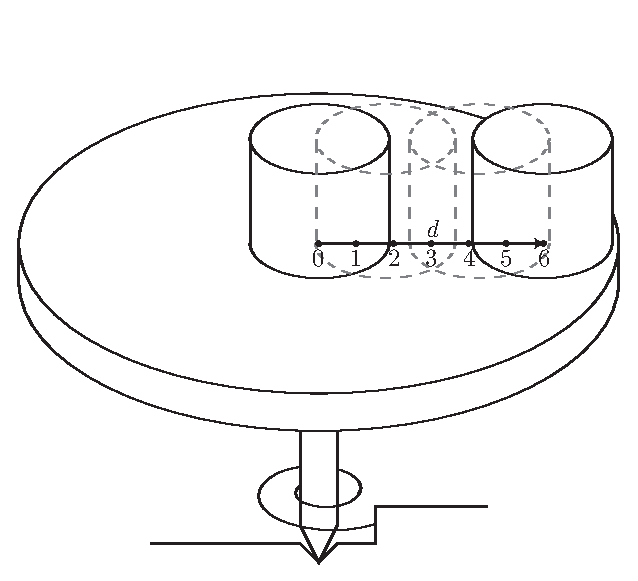
\includegraphics[width=10cm]{illustration3.pdf}
\end{center}
Ein Zylinder ($m$ = 300g, $r$ = 2cm) wird zuerst zentral auf dem Drehtisch montiert und dann schrittweise jeweils 1 cm zum Rand bewegt bis er insgesamt 6cm vom Zentrum entfernt ist. Bei jedem Schritt wird die Periode $T$ wie bisher gemessen, anstatt zehn werden aber nur je f\"unf Messungen durchgef\"uhrt.

% Rohdaten
\subsection*{Rohdaten}
\begin{tabular}{|l|r|r|r|r|r|r|}
\hline
$d$&$T_1$&$T_2$&$T_3$&$T_4$&$T_5$&$10\overline{T}$\\
\hline
0cm&12.4s&12.3s&12.4s&12.65s&12.45s&12.44s\\
1cm&12.55s&12.7s&12.75s&12.7s&12.55s&12.65s\\
2cm&12.4s&13.55s&13.25s&13.4s&13.25s&13.17s\\
3cm&14.5s&14.5s&14.4s&14.5s&14.5s&14.48s\\
4cm&16s&15.8s&15.8s&16s&16.05s&15.93s\\
5cm&17.6s&17.55s&17.7s&17.65s&17.5s&17.60s\\
6cm&19.35s&19.5s&19.7s&19.45s&19.45s&19.49s\\
\hline
\end{tabular}

% Auswertung
\subsection*{Auswertung}
\subsubsection*{Grafische Darstellung}
Um den Zusammenhang zwischen $d$ und $J$ besser zeigen zu k\"onnen bilden wir ab auf $x = d^2$ und $y = T^2$.
Die Regressionsgerade l\"asst sich nach Formel 1.27 aus dem Skript wie folgt berechnen:
\[ s_{xy} = \frac{1}{N - 1}\sum_{i=1}^{N}(x_i - \overline{x})(y_i - \overline{y}) =  0.001148 \]
\[ s_x^2 = \frac{1}{N - 1}\sum_{i=1}^{N}(x_i - \overline{x})^2 =  1.82\cdot 10^{-6} \]
\[ \hat{y} = \frac{s_{xy}}{s_x^2}(x - \overline{x}) + \overline{y} = 630.35x + 1.5252 \]
\begin{center}
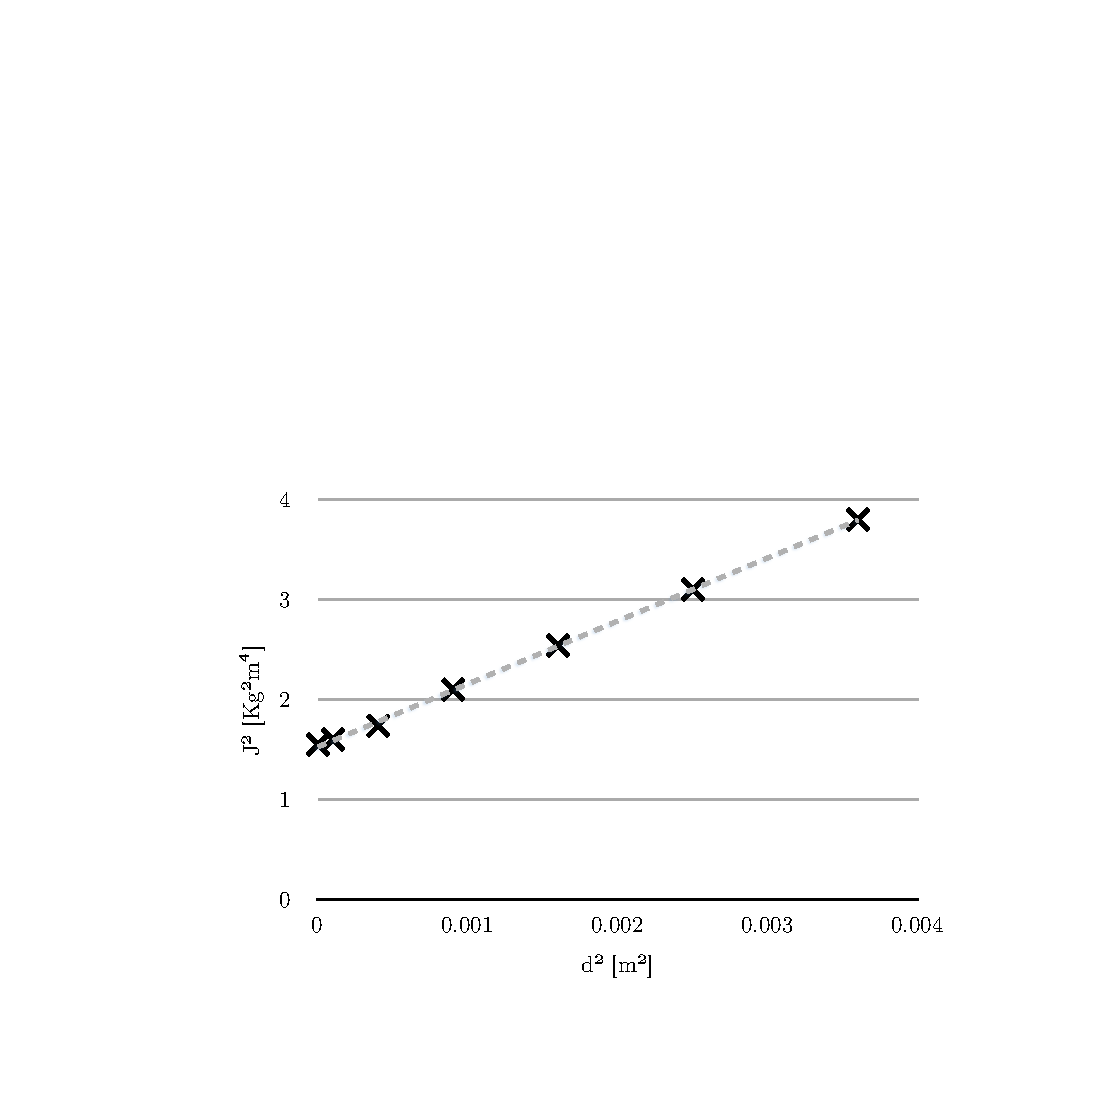
\includegraphics[width=10cm]{diagram.pdf}
\end{center}

\noindent
Der Achsenabschnitt der Geraden entspricht ${T_0}^2$, die Steigung h\"angt von $m$ und $k$ ab:
\[ \frac{\Delta T^2}{\Delta d^2} = \frac{4m\pi^2}{k} \]

\newpage
\subsubsection*{Satz von Steiner}
Der Satz von Steiner besagt, dass sich das Tr\"agheitsmoment $J$ eines K\"orpers nach einer Verschiebung senkrecht zur Drehachse um $md^2$ erh\"oht, wobei $d$ die Distanz zur Urspr\"unglichen Drehachse beschreibt. Das Tr\"agheitsmoment jeder Position des Experiments l\"asst sich nach Formel \ref{eq:k} berechnen:

\vspace{15pt}
\begin{tabular}{|l|l|l|l|}
\hline
$J_{0}$&$J_{1}$&$J_{2}$&$J_{3}$\\
\hline
0.000069kgm${}^2$&0.000093kgm${}^2$&0.000154kgm${}^2$&0.000319kgm${}^2$\\
\hline
\end{tabular}

\begin{tabular}{|l|l|l|}
\hline
$J_{4}$&$J_{5}$&$J_{6}$\\
\hline
0.000520kgm${}^2$&0.000775kgm${}^2$&0.001094kgm${}^2$\\
\hline
\end{tabular}

\vspace{15pt} \noindent
Wendet man den Satz von Steiner auf den jeweils vorherigen Wert an erh\"alt man folgende Tr\"agheitsmomente:

\vspace{15pt}
\begin{tabular}{|l|l|l|}
\hline
$J_{1}$&$J_{2}$&$J_{3}$\\
\hline
0.000099kgm${}^2$&0.000189kgm${}^2$&0.000339kgm${}^2$\\
\hline
\hline
$J_{4}$&$J_{5}$&$J_{6}$\\
\hline
0.000549kgm${}^2$&0.000819kgm${}^2$&0.001149kgm${}^2$\\
\hline
\end{tabular}

\vspace{15pt} \noindent
Die jeweilige Abweichung betr\"agt:

\vspace{15pt}
\begin{tabular}{|l|l|l|}
\hline
$\Delta J_{1}$&$\Delta J_{2}$&$\Delta J_{3}$\\
\hline
6.48\%&22.65\%&6.20\%\\
\hline
\hline
$\Delta J_{4}$&$\Delta J_{5}$&$\Delta J_{6}$\\
\hline
5.55\%&5.64\%&4.96\%\\
\hline
\end{tabular}

%%
% Diskussion
%%
\section*{Diskussion}
Die experimentell ermittelten Tr\"agheitsmomente aus Experiment 2 weichen nur ca. 5\% vom theoretischen Wert ab. Die Messungen waren so genau, da jeweils 10 Perioden und nicht nur eine Periode gemessen wurden.
Die in Experiment 1 berechnete Federkonstante wurde in den n\"achsten Experimenten weiter verwendet. Durch die darauffolgenden kleinen Abweichung aus Experiment 2 l\"asst sich schliessen, dass diese Federkonstante sehr genau bestimmt wurde.
Im dritten Experiment wurde der Satz von Steiner verifiziert. Die Abweichung betr\"agt nur in einem Fall \"uber 20\%, sonst jeweils unter 7\%.

\end{document}